In order to understand, according to what already said, what a SNP can cause, we must first of all \emph{identify the SNP in the DNA} of the subject under consideration.
\\
\\There are many possible types of analysis that can be performed (DNA sequencing, capillary electrophoresis, mass spectrometry, electrochemical analysis, ...); in this essay we will look at the most common one: \textbf{DNA Sequencing}.
\\
\\
\\\emph{“DNA Sequencing is the process of determining the precise order of nucleotides within a DNA molecule. It includes any method or technology that is used to determine the order of the four bases — adenine, guanine, cytosine, and thymine — in a strand of DNA.”}

\vspace{15mm}

\section{History of DNA Sequencing}

Over the years, since the discovery of DNA by \emph{Miescher} in 1870, the problem of DNA sequencing has been addressed in an increasingly thorough (see \emph{Figure 3.1}). This also because, in 1940, \emph{Avery} realized, by means of an experiment, that the so-called \emph{transforming principle} (the carrier of genetic information) discovered in 1928 by Griffith was DNA.

\vspace{15mm}

\begin{figure}[ht!]
	\centering
	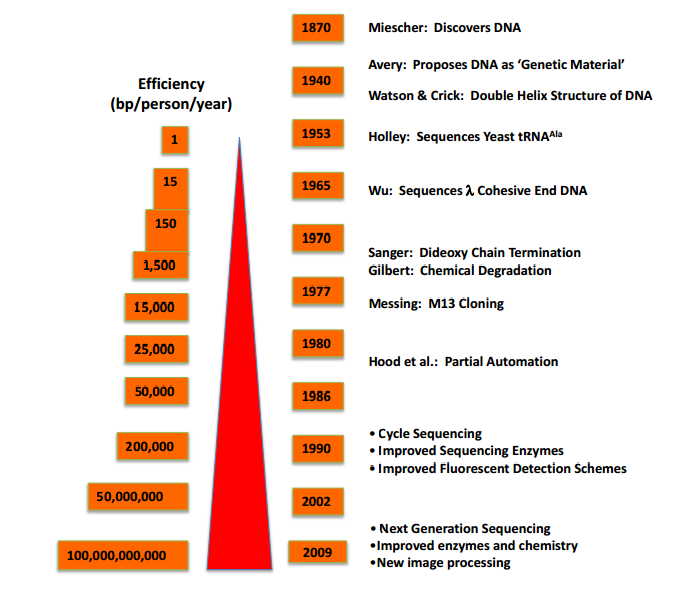
\includegraphics[width=150mm]{../Images/DNASequencing_history.png}
	\label{overflow}
	\caption{History of DNA Sequencing}
	\end{figure}


\newpage

\subsection{Avery’s experiment}

In short, the Avery experiment was based on the Griffith experiment. Griffith used in his studies the \emph{Streptococcus pneumoniae}. In particular, two of its strains:

\begin{itemize}
	\item the S strain, which can cause pneumonia in guinea pigs (virulent strain)
	\item the R strain is not able to cause pneumonia in guinea pigs (avirulent strain)
\end{itemize}

The main result was this:
\\
\\injection in mouse of type S bacteria, killed after thermal treatment, and type R live bacteria was able to cause disease and death of the animal. From the tissues of mouse could isolate live bacteria of the S strain.
\\
\\
\\So, he verified and demonstrated that in a mixture containing either S dead bacteria and R alive bacteria, were to be happened the exchange of some substance (genetic material) that would confer virulence to bacteria R (which were then transformed into S).
\\
\\
\\The experiment of Avery aimed to determine what this substance was and it was discovered that it would necessarily be DNA. 

\subsection{Progress over the years}

\begin{wrapfigure}{l}{0.2\textwidth} %this figure will be at the right
    \centering
    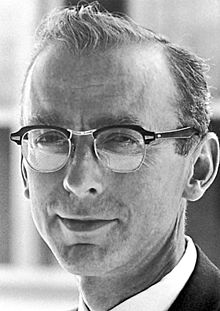
\includegraphics[width=0.2\textwidth]{../Images/RobertWHolley.jpg}
    \label{overflow}
\end{wrapfigure}

The first sequencing occurred in 1953 by Holley.
\\
\\Since then, the efficiency of sequencing increased exponentially over the years: if in 1953 a person in a year could sequence only one \emph{bp} (base pair), in the seventies we get to more than 1,500, in the nineties to more than 200000 and few years ago, in 2009, to more than 100 billion bps!

\vspace{5mm}

The first full DNA genome to be sequenced was that of a bacteriophage in 1977. Medical Research Council scientists deciphered the complete DNA sequence of the Epstein-Barr virus in 1984, finding it to be 170 thousand base-pairs long.

\subsection{Sequencing methods}

Over the years, many methods have been developed for sequencing the DNA. It goes from \textbf{basic methods}, such as the \emph{Maxam-Gilbert sequencing} and \emph{Chain-termination methods}, to \textbf{advanced methods} such as the \emph{Shotgun sequencing} or \emph{PCR Bridge}, to get to the \textbf{next-generation methods} (\emph{Massively Parallel Signature se-quencing (MPSS), Polony sequencing, 454 pyrosequencing, Illumina (Solexa) sequencing, SOLiD sequencing, Single Molecule Real Time (SMRT) sequencing, ...)}.

\subsection{Next-Generation Sequencing}

Nowadays, thanks to technological progress we pushed even further forward. As can be seen from the following chart, it is possible to sequence \textbf{more than 100 million base pairs in about a week} (generating a very high amount of data). This is called the \textbf{Next-Generation Sequencing}.
\\
\\
\\However, the higher the speed of sequencing, the more there is a problem:  \textbf{interpretation}. It often represents a real bottleneck; a single computer is not able to interpret a sequencing at the same speed of which it is presented to him.
\\
\\For this reason, usually \emph{cloud computing} services are used. They allow to take advantage of the computing power of multiple computers at the same time, parallelizing the work and thereby reducing the overall time.

\vspace{30mm}

\begin{figure}[ht!]
	\centering
	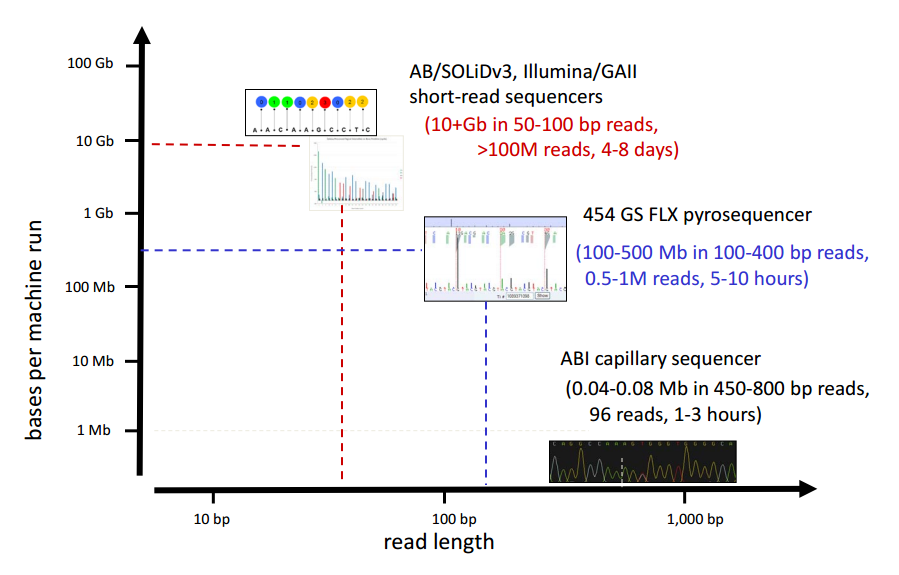
\includegraphics[width=150mm]{../Images/NowadaysSequencing.png}
	\label{overflow}
	\caption{Nowadays Sequencing}
	\end{figure}

The high demand for low-cost sequencing has also driven the development of high-throughput sequencing (or next-generation sequencing) technologies that parallelize the sequencing process, producing thousands or millions of sequences concurrently. High-throughput sequencing technologies are intended to \emph{lower the cost of DNA sequencing} beyond what is possible with standard methods.
\\In ultra-high-throughput sequencing as many as 500,000 sequencing-by-synthesis operations may be run in parallel.
\\
\\
\\Although each next-generation sequencing platform is unique in how sequencing is accomplished, there is a similar base methodology that includes preparation, sequencing, and data analysis. Within each generalized step, the individual platforms have unique aspects.
\\
\\The common work-flow is the following:

\begin{figure}[ht!]
	\centering
	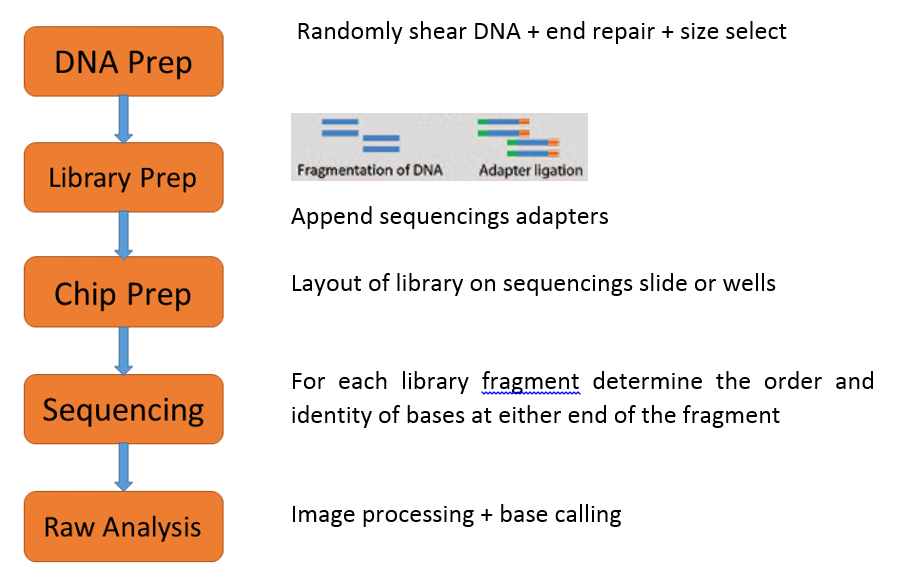
\includegraphics[width=150mm]{../Images/NGSworkflowCommented.png}
	\label{overflow}
	\caption{Nowadays Sequencing}
	\end{figure}


\section{DNA Sequencing Data format}

Text



\section{SNPs databases}

Because SNPs are expected to facilitate large-scale association genetics studies, there has recently been great interest in SNP discovery and detection. For this reason databases can to serve as a central repository. Once discovered, polymorphisms could be used by additional laboratories, using the sequence information around the polymorphism and the specific experimental conditions.
\\
\\
\\There are several databases that, nowadays, are used. The most important are:

\begin{enumerate}
	\item \textbf{dbSNP}, a SNP database from the \emph{National Center for Biotechnology Infor-mation (NCBI)}
	\item \textbf{SNPedia}, a wiki-style database supporting personal genome annotation, interpretation and analysis
	\end{enumerate}

Furthermore, there are various support database that allow, for example, to bind a SNP to the disease that causes:

\begin{enumerate}
	\item \textbf{OMIM} database describes the association between polymorphisms and diseases (e.g., gives diseases in text form)
	\item \textbf{Human Gene Mutation Database} provides gene mutations causing or associ-ated with human inherited diseases and functional SNPs
	\item \textbf{GWAS Central} allows users to visually interrogate the actual summary-level association data in one or more genome-wide association studies
	\item \ldots
	\end{enumerate}